\scanpage{23}
Nous attachons maintenant notre attention à la condition f). \deleted{Il est clair}\inserted{On a vu} qu'elle \deleted{\unsure{est}} est stable par restriction à un ouvert $\in F$, mais il est assez clair qu'elle n'est pas stable par restriction à un ouvert quelconque. On a seulement, alors, que si $A\in\overline F_U$ est loc fermé dans $U$ (donc \unsure{l'est|fermé} dans un ouvert plus petit $V\subset U$), alors $A$ est loc. connexe, \deleted{et $\unsure{\overline F|F}$} donc ses comp. connexes sont ouvertes. Si $A$ est loc compact (p.ex. si $X$ l'est) alors ses comp. connexes \unsure{forment} donc une famille loc finie dans $A$ (donc dans $V$) \deleted{\unsure{mais est}} \uline{Elle} \inserted{\uline{est $=$}} \uline{\unsure{loc$^t$} finie dans} $U$?
\margin{Je suppose la top. de $X$ engendrée par les ouverts $\in F$}

\deleted{\unsure{Cela n'est que} au voisinage de tt pt de $U$, on a $A=\deleted{\unsure{Z\cap U}}$ avec $\deleted{\unsure{B}}Z\in F$ $Z$ loc. fermé,} car $\forall x\in U$, $\exists$ voisinage ouvert $V\in F_U$, tel que $A\cap V\in F$, et $A\cap V$ n'a qu'un nb fini de comp connexes.

\figure{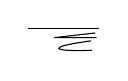
\begin{tikzpicture}[x=1cm,y=1cm]\draw (-.45,.12)--(.45,.12);\draw (.4,.06)--(-.12,0)--(.42,0);\draw (.35,-.04)..controls(-.25,-.12)and(-.15,-.18)..(.36,-.16);\end{tikzpicture}}

Soit $\underline F$ un sous-faisceau du faisceau $\underline{\mathcal P}_X$ des germes de parties de $X$. On suppose que $\underline F$ satisfait a) b) c) d), et \deleted{\unsure{que de plus une famille}} \inserted{e)} Soit $U$ un ouvert de $X$, et $X_1\supset X_2\supset\cdots\supset X_n\supset\cdots$ des fermés de $U$, $\in\Gamma(U,\underline F)$, tels que $X_{\unsure{n+2|n+1}}$ rare dans $X_n$. Alors la suite des $X_i$ est loc finie sur $U$, donc $\bigcap X_i=\varnothing$.
\mspage{24}
